\section{Ordered Sets}
\begin{definition}
	A totally ordered set is a set $S$ plus a relation $R$ on the set (called a total
	order) that satisfies the conditions for a partial order plus an additional
	condition known as the comparability condition. A relation $\geq$ is a total order
	on a set $S$ ($\geq$ totally orders $S$) if the following properties hold.
	\setcounter{equation}{0}
	\begin{align}
		a\leq a, \forall a \in S                &  & \text{reflexive}     \\
		a\leq b \land b\leq a \implies a=b      &  & \text{antisymmetric} \\
		a\leq b \land b\leq c \implies a\leq c  &  & \text{transitive}    \\
		\forall a,b \in S, a\leq b \lor b\leq a &  & \text{trichotomy}
	\end{align}

\end{definition}
\subsection{Totally Ordered Set}
A totally ordered set defines a category $\mathcal{C}$ where $\forall a, b \in
	\obc{}$, there is exactly one arrow between them.

\subsubsection{Example}
\begin{align*}
	A=                     & \set{S, M, L, XL}                    \\
	R\subseteq A\times A = & \set{(S, S), (S, M), (S, L), (S, XL) \\
	                       & (M, M), (M, L), (M, XL)              \\
	                       & (L, L), (L, XL)                      \\
	                       & (XL, XL)
	}
\end{align*}
\begin{figure}[H]
	\begin{center}
		\documentclass{standalone}
\usepackage{tikz}
\begin{document}
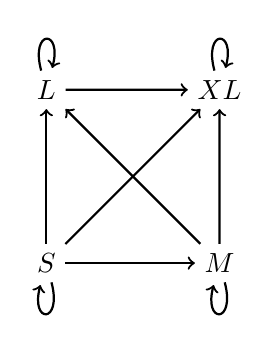
\begin{tikzpicture}[scale=1.1]
	\tikzset{arc lines/.style={thick,black, ->}}
	\node (S) at (0, 0) {$S$};
	\node (M) at (2, 0) {$M$};
	\node (L) at (0, 2) {$L$};
	\node (XL) at (2, 2) {$XL$};
	\draw [arc lines] (S) to (M);
	\draw [arc lines] (S) to (L);
	\draw [arc lines] (S) to (XL);
	\draw [arc lines] (M) to (L);
	\draw [arc lines] (M) to (XL);
	\draw [arc lines] (L) to (XL);
	\path [-stealth, thick]
	(S) edge [loop below] (S)
	(M) edge [loop below] (M)
	(L) edge [loop above] (L)
	(XL) edge [loop above] (XL)
	;
\end{tikzpicture}
\end{document}

	\end{center}
	\caption{Corset toset}
\end{figure}
Notice there is indeed exactly one arrow between any two elements. If an
arrow can be reversed, it is the identity arrow.

\begin{ttta}
	Check there is only one arrow between any two objects for the category of $\mathbb{N}$ with the relation $\geq$.
\end{ttta}
\begin{proofitem}
	\item Let $T$ be a totally ordered set.
	\item Let $R\subseteq T\times T$ be a total order on $T$.
	\item Let $\mathcal{C}$ be a category, where each $t\in T$ is an
	object $o\in\mathcal{C}$.
	\item For any two distinct objects $a, b\in\obc{}$, there will be one arrow
	between $a$ and $b$ because $T$ is antisymmetric, and therefore if $x, y \in
		T$, only one of $(x, y)$ and $(y, x)$ can be in $T$.
	\item For any object $a\in\obc{}$, there will exist an identity arrow because
	$T$ is reflexive.
	\item Therefore we have shown there is only arrow between objects $a, b\in
		\obc{}$ when $a=b$ and when $a\neq b$.
\end{proofitem}

\stepcounter{tttacounter}
\begin{ttta}
	How many ways can you think of for a category to fail to be an
	ordered set?
\end{ttta}
\begin{proofitem}
	\item For a category to be an ordered set there must be one arrow between any
	pair of objects. Therefore a category can fail to be a totally ordered set
	if there are 0 arrows between two objects, or if there is more than 1 arrow
	between two objects.
\end{proofitem}

\subsection{Partially Ordered Set}
\setcounter{tttacounter}{6}
\begin{ttta}
	In Chapter 5 we moved from lattices of factors to lattices of subsets.
	Can you make a formal definition of a category of subsets of S (for some fixed
	set S, based on \S 5.6? Can you then show that it is a poset?
\end{ttta}
\begin{figure}[H]
	\begin{center}
		\documentclass[border=0.2cm]{standalone}
\usepackage{tikz}
\usepackage{titlesec}
\usepackage{float}
\usepackage{standalone}
\usepackage{tikzit}
\usetikzlibrary{automata, arrows.meta, positioning}
\usetikzlibrary{arrows.meta, positioning}
\input{sample-02.tikzstyles}

\begin{document}
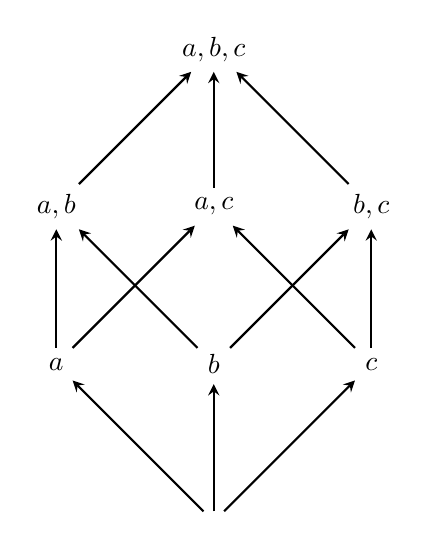
\begin{tikzpicture}[->, >=stealth, thick]
\node (1) at (4,0) {$\varnothing$};
\node (2) at (2,2) {$\set{a}$};
\node (3) at (4,2) {$\set{b}$};
\node (5) at (6,2) {$\set{c}$};
\node (6) at (2,4) {$\set{a, b}$};
\node (10) at (4,4) {$\set{a, c}$};
\node (15) at (6,4) {$\set{b, c}$};
\node (30) at (4,6) {$\set{a, b, c}$};
\draw (1) -- (2);
\draw (1) -- (3);
\draw (1) -- (5);
\draw (2) -- (6);
\draw (2) -- (10);
\draw (3) -- (6);
\draw (3) -- (15);
\draw (5) -- (10);
\draw (5) -- (15);
\draw (6) -- (30);
\draw (10) -- (30);
\draw (15) -- (30);
\end{tikzpicture}
\end{document}

	\end{center}
	\caption{Subset Lattice}
\end{figure}
\begin{proofitem}
	\item The subsets of $S$ are represented be the powerset $\mathscr{P}(S)$.
	\item Let $\mathcal{C}_\text{subset}$ be the category of subsets for a set $S$.
	\item The objects $\obc{}$ of $\mathcal{C}_\text{subset}$ are the elements of
	the powerset $\mathscr{P}(S)$.
	\item An arrow exists from $a$ to $b$ if $a\subseteq b$.
	\item For $\mathcal{C}_\text{subset}$ to be a poset, it must have the following
	properties: reflexivity, transitivity, and anti-symmetry.
	\setcounter{equation}{0}
	\begin{align}
		A \in \mathscr{P}(S) \implies A\subseteq A                            &  & \text{reflexivity}  \\
		A,B \in \mathscr{P}(S), A\subseteq B \land B \subseteq A \implies A=B &  & \text{antisymmetry} \\
		A,B,C \in \mathscr{P}(S), A \subseteq B \land B \subseteq C \implies A
		\subseteq C                                                           &  & \text{transitivity}
	\end{align}
	\item Thus we have shown that $\mathcal{C}_\text{subset}$ is a poset.
\end{proofitem}
